% !TEX root = ANA-GENR-2018-01-INT1.tex
% Turn off some chktex warnings.
% chktex-file 1 chktex-file 8 chktex-file 46

%------------------------------------------------------------------------------
\section{ATLAS work strategy}%
\label{sec:ATLAS_work_strategy}
%------------------------------------------------------------------------------

%------------------------------------------------------------------------------
\subsection{ATLAS analyses and publications}%
\label{sec:The_ATLAS_Analyses_and_Publications}

The main objective of \GSnote{ATLAS is research}{physics research in ATLAS, but really, this shouldn't be super detailed and you should rephrase this paragraph to say that you need to support the general physics programme of ATLAS} to explain the nature of matter,
% (from ancient Greek  phusikós),
as well as to look for new phenomena and decay channels.
To explain nature, it makes use of the gigantic hadron accelerator (LHC),
which collides protons at almost the speed of light.
With the centre-of-mass energy of \SI{13}{\TeV} provided by the accelerator, we explore matter, its interaction, its properties and simulate small big bangs every second.
Millions of particles collide in the accelerator and the ATLAS experiment is there to spy the evolution of these mini big bangs and try to make the most accurate interpretation.
The results of this research complement our understanding of the nature of matter and the evolution of the universe.
This information is recorded using mathematical \GSnote{tools}{tools?}, in the \GSnote{so called}{remove} Standard Model and many other theoretical models.
\IBnote{}{I think we have to rethink what we want to say here. Our data analysis is not recorded in the SM.}

To perform such a physics program, physicists need \GSnote{tools}{tools?} to analyse the data and compare them to the different models on the market.
For this, ATLAS is organised in several physics (PHY) and \GSnote{so-called}{remove} Combined Performance (CP) groups and \GSnote{subgroups}{subgroups of what? PHY or CP or both?}.
These groups are coordinated by conveners,
who are elected or appointed by the collaboration for one or more years.
The physics and CP \GSnote{leading}{???} groups are, for example, top quark (TOPQ), Standard Model (STDM), \PB physics (BPHY), Higgs (HIGG), Electron/Gamma (EGAM), Jet and \GSnote{Etmiss}{EtMiss} (JETM) \GSnote{etc}{??? we know all the current groups...}.
Further studies on system detectors (SYS) or other activities like software (SOFT) and data preparation (DAPR) are also organised \GSnote{in leading groups and subgroups with conveners}{hierarchically with subgroups and conveners}.

Once an analysis is finished or an aspect of the detector performances has been studied in detail,
the \GSnote{physicist}{analysis team} is asked to prepare a publication.
In fundamental research, as is the case with the research conducted at CERN, the communication to the public is not only compulsory but is the \IBnote{exclusive}{In what sense exclusive?} way to demonstrate and show the results.

ATLAS considers three different types of publications:\GSnote{}{This should be a bulleted or enumerated list} general publications based on data and the project-related publications (PAPER), public documents classified as notes (PUB notes), and conference proceedings (PROC) or notes (CONF Notes) on preliminary results, which are shown at conferences.

All ATLAS analyses are discussed and presented in the relevant working groups \GSnote{}{Something more about how each group internally governs the process before it reaches PC/PubComm/etc...} (physics, combined performance, systems and detectors, etc.). The Physics Coordinator, the working groups conveners and the Publication Committee members are informed of all ongoing analyses and publications. They also appoint analysis contacts, contact editors\GSnote{}{,} and review experts.
When the paper draft \IBnote{is ready}{The EdBoard is set up before this},
they set up an Editorial Board, set meetings dates to review the analysis and \IBnote{the goal}{They do not really review the goal} of that analysis (CONF note, PAPER or PUB note). \GSnote{}{There's a document from PubComm that describes this entire process that should be cited here: https://cds.cern.ch/record/1980862 or something?}

\IBnote[inline]{}{Some discussion of the phases needs to be added here,
so that the following makes sense}
\GSnote{Pull in information from https://cds.cern.ch/record/1980862 or figure out a way to get parts of it public, or if the difficulty is that these recommendations/procedures are in flux}

%------------------------------------------------------------------------------
\subsection{Author lists, Acknowledgments and Proof Checker}%
\label{sec:Authorlists_acknowledgments_and_ProofChecker}

Author lists and Acknowledgements are two of the final steps of a paper’s publication and both are handled and generated, using the FENCE framework, described in detail in \cref{sec:The_FENCE_project}.
After the papers containing the author lists and acknowledgements are submitted to the journals,
they come back to the ATLAS Physics Office for a final review before the publication.
This review is mainly performed automatically using a PO tool: the Proof Checker.

The author list is the inventory of qualified authors at a given date, which is also called the reference date. Every paper has a related list of qualified authors with a reference date which corresponds to the creation date of that list at the Paper Phase 1, just before the first circulation to the collaboration. Qualified authors are active physicists, still contributing to the maintenance and the operations of the collaboration.
Some of them are retired people benefiting from their pre-data credits (worked before the data era), called signing-only authors.
Between FENCE Phase 1 and Phase 2 (\GSnote{second circulation to the collaboration}{Phase 1/Phase 2 should be in parens because the people reading this document are not PO experts and care more about the qualitative meaning of the phases, not the phase itself}), some people may get exceptional authorship because of their involvement in the analysis or the paper,
even if they are not yet a qualified author.
Therefore the author list is updated to include \enquote{exception} authors.
The special cases are studied by the Authorship Committee and proposed for approval to the \GSnote{}{ATLAS }Spokesperson.

All this information is stored in the ATLAS database and managed by FENCE\@.
\Cref{fig:authorlist_generation} shows a the start of the full list of members (active and retired), their institutes and the related metadata that is needed to generate a full report of members and institutes.

\begin{figure}[htb]
  \centering
  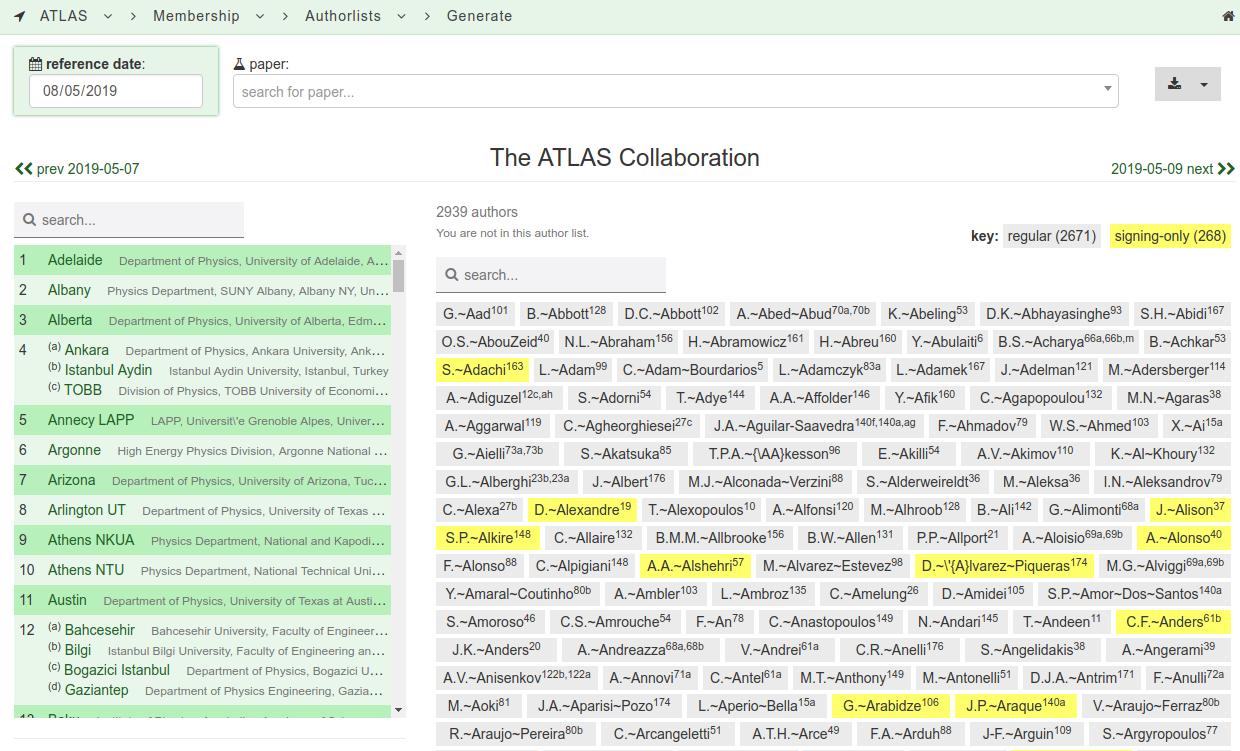
\includegraphics[width=0.9\textwidth]{figures/authorlist_generation.png}
  \caption{FENCE author list generation interface. \GSnote{}{Please expand the caption more to include explanation of the different piecces of the screen. Why are some names yellow? What's the green stuff on the left? Who can access this interface?}}%
  \label{fig:authorlist_generation}
\end{figure}

The acknowledgements are a legal paragraph that the collaboration agrees to add in each paper to thank \GSnote{Funding Agencies and Foundations}{shouldn't be capitalized, also in other places following this...} for their financial support.
They do not change very often, but may include or suppress a Funding Agency or Foundation at a given date.
Therefore, an acknowledgement file is built for each paper at a specific date, which is called the reference date.

The proof checker is a tool provided mainly for the ATLAS PO members to compare the final publication (PDF file) of author lists and acknowledgement provided by the journal with ATLAS data (XML file). The main purpose of the proof checker is to identify inconsistencies between data provided to the journal and what the journal will produce as final output. A report of this comparison, one for every version of the proof, is available to the ATLAS PO members so they can check the results.

\GSnote{}{Expand more on proof checker? Shouldn't you have three subsections here? One discussing the FENCE interface for author lists, one that discusses more about how the acknowledgements are generated -- explaining that they're reviewed by a legal team if at all, and more about how that's generated; and more about the proof checker. Is it a script? How is it almost fully-automated? Does someone run it or is it automatically run? What's the example output, etc...?}
